\chapter{Environment}
\label{chapter:environment}

The developed thesis project is based on a major environment that comprises multiple structures.
First of all, the Middlebury 2014 \cite{Scharstein2014} dataset, which contains detailed stereo pairs, was exploited to perform multiple tests.
Moreover, real indoor rectified stereo images taken with the \textbf{company cameras} were employed.\\
In this chapter a brief explanation of the LaDimo stereo device follows.
Furthermore, it is worth to describe the main characteristics of the dataset adopted.
As a matter of fact, it results extremely useful during the overall designing of the implementation, giving visual outcome of the improvement provided to the code.
The ground truth images available in the dataset were especially effective for simulating the behaviour of the company device during the first part of the code implementation.

\section{Middlebury Dataset}
\label{section:middledataset}

The so called Middlebury 2014 dataset is a high-resolution stereo dataset comprising static indoor scenes and including highly detailed ground-truth disparities.
The images were acquired exploiting a novel structured lighting system.
This also consists of updated methods for accurate 2D subpixel correspondence search and self-calibration of camera and projectors with modelling of lens distortion.\\
Generally speaking, Scharstein et al. \cite{Scharstein2014} provide 33 new indoor 6-megapixel datasets using their system. 
Thus, achieving an accuracy in the disparity estimation of 0.2 pixels on most analysed surfaces, they produce demanding challenges for the stereo algorithms developed since that.\\
That was, in fact, one of their main objective, being the datasets available until their work insufficient in terms of ground truth accuracy, resolution, complexity and realism. 
Therefore, aiming at updating and improving the work of Scharstein and Szeliski \cite{scharstein2003high}, they obtained Middlebury 2014 dataset, which brought major improvements in the level of calibration accuracy for stereo images.\\
Specifically, the system described in \cite{Scharstein2014} comprises the following novel features: 
\begin{itemize}
	\item a stereo equipment made of two digital single-lens reflex (DSLR) cameras and two point-and-shoot cameras;
	\item a method for robust interpolation of lighting codes and 2D subpixel correspondence search for obtaining accurate floating-point disparities;
	\item bundle adjustment for calibration and rectification procedures;
	\item a robust model selection for self-calibration of structured light projectors and lens distortion;
	\item a so called \textit{imperfect} version of the dataset showing realistic rectification errors.
\end{itemize}  
Figure \ref{fig:dataset-example} shows an examples of the datasets provided, which comprise the input images, with different levels of exposure, and \textit{perfect} and \textit{imperfect} rectified images with accurate 1D and 2D floating-point disparities, respectively. 
 
\begin{figure}[t]
	\centering
	\subfigure[Left Stereo Image Example]{
 		\includegraphics[width=0.4\textwidth]{images/im0.png}
}
	\subfigure[Disparity Left Image Exaple]{
 		 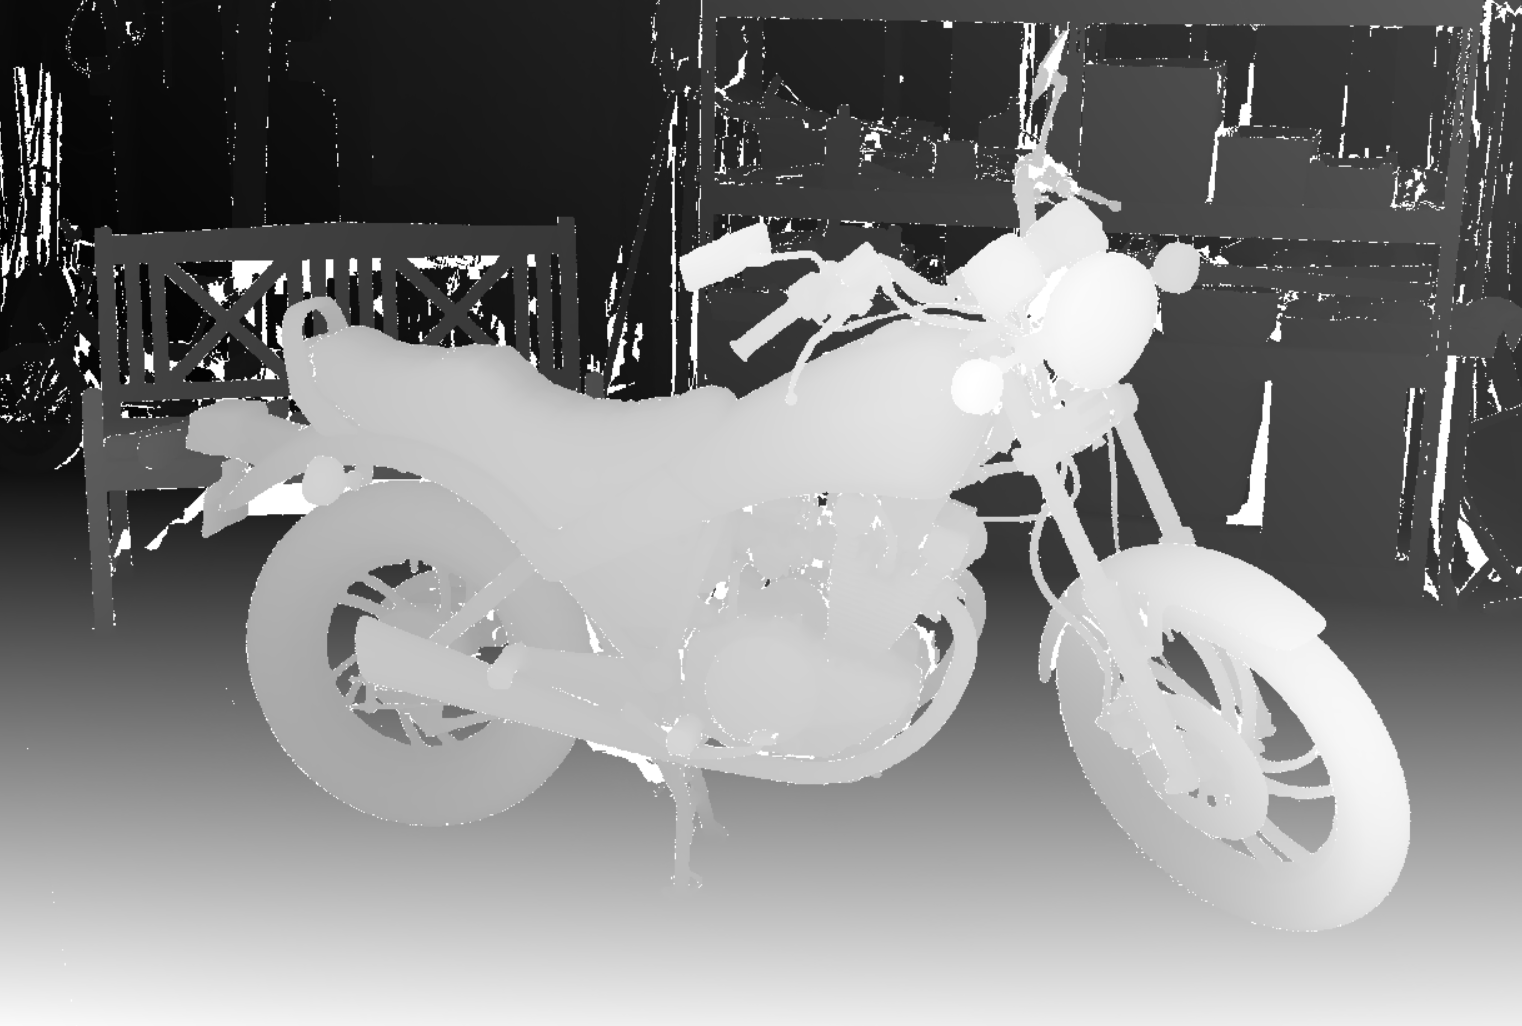
\includegraphics[width=0.4\textwidth]{images/im-0-disp.png}
}
\caption{Middlebury 2014 dataset example}
\label{fig:dataset-example}
\end{figure}

In order to obtain accurate high-resolution stereo datasets, the authors of the described work based their idea on establishing ground-truth disparities from the input views.
In this manner, calibration problem are prevented and the process can be performed via structured light.
However, the drawback of this is that correct disparities can be achieved only for scene points that are non-occluded in both images.
Therefore, extending the idea in \cite{scharstein2003high}, that is based on a self-calibration of structured light sources from initial non-occluded disparities, they managed to register illumination disparities in half-occluded regions and model projector lens distortion as well. 
Moreover, imposing initial correspondences they enhance significantly the rectification accuracy.
Then, subpixel precision was obtained exploiting a high number of binary patterns under multiple exposures and applying a robust interpolation.\\
A brief overview of the pipeline of the process, deeply illustrated in \cite{Scharstein2014}, is now presented.\\

\begin{figure}[t]
	\begin{center}
		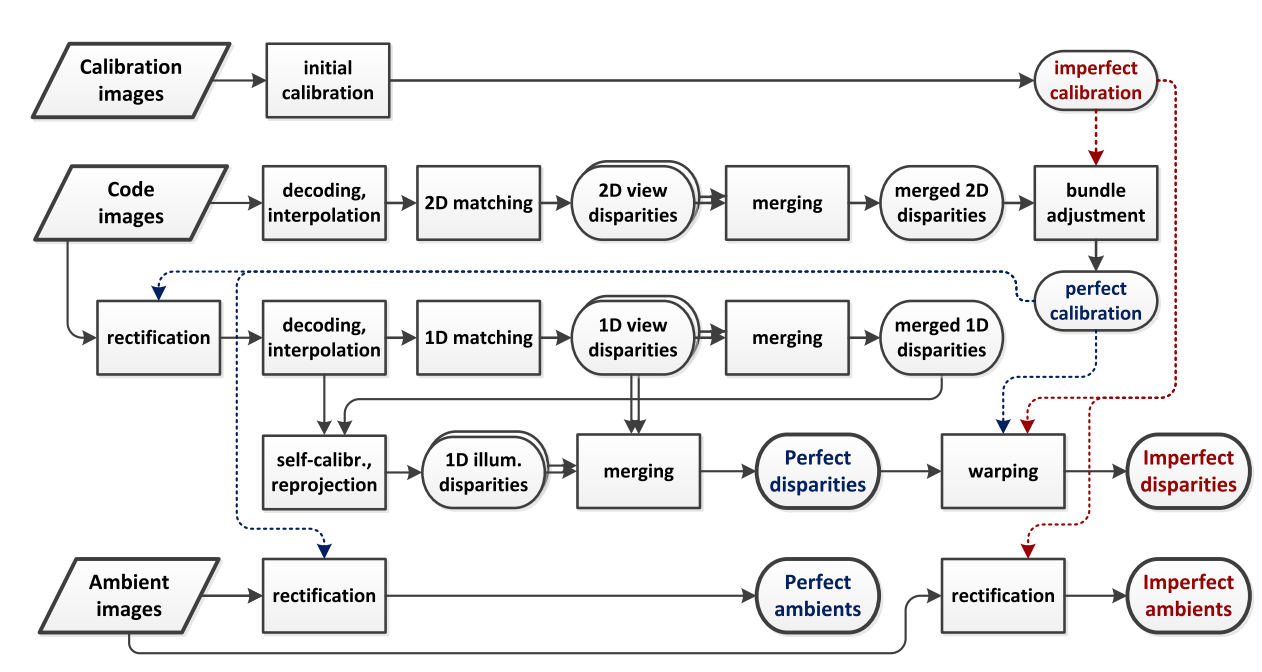
\includegraphics[width=.8\textwidth]{images/middlebury-2014-pipeline.png}
		\caption{Pipeline of the overall system for creating the Middlebury 2014 dataset \cite{Scharstein2014}}
		\label{fig:middleury-pipeline}
	\end{center}
\end{figure}

Figure \ref{fig:middleury-pipeline} depicts the overall pipeline of the system defined by Scharstein et al. \cite{Scharstein2014} for reconstruct the stereo datasets.\\
As simply described, the system's inputs are: calibration images of a standard checker-board calibration target; code images obtained with structured lighting projectors from different positions; \textit{ambient} images collected with multiple lighting conditions. 
First of all, re-factoring operations are applied to the unrectified code images, i.e. thresholding, decoding and interpolation.
This leads to floating-point coordinates of the projector pixel illuminating the scene. 
Thus, the achieved values are employed as unique identifiers to impose the correspondences between the two input images. 
So that, the resulting \textit{2D view disparities} are used to refine the \textit{imperfect} calibration in the bundle-adjustment phase.
The next step of the process is use the rectified input images to generate the \textit{1D view disparity}.
The self-calibration of the projector is, therefore, accessed using the merged disparities and thereby produce the \textit{1D illumination disparities}.
View and illumination disparities are, then, combined together into the \textit{perfect} disparities. 
Last row in Figure \ref{fig:middleury-pipeline} shows that rectifying with both calibration allows to achieve the corresponding sets of ambient images.\\
Further details of the single steps of the process are reminded to the original paper \cite{Scharstein2014} so as not to make the discussion much convoluted.\\
Nevertheless, it is worth to disclose that considering the evaluation of the datasets showed in \cite{Scharstein2014}, the choice of the Middlebury 2014 images for the initial tests can be assumed as a correct decision.
As a matter of fact, experimental results reported in the original paper demonstrate how that datasets can be considered highly challenging in terms of accuracy and scene complexity.
Therefore, they can be assumed as a useful starting point for recovering information from the ground truth images available and for the stereo algorithm evaluation.\\

\section{Stereo Photogrammetry Ladimo device}
\label{section:stereo-device}

\begin{figure}[t]
	\begin{center}
		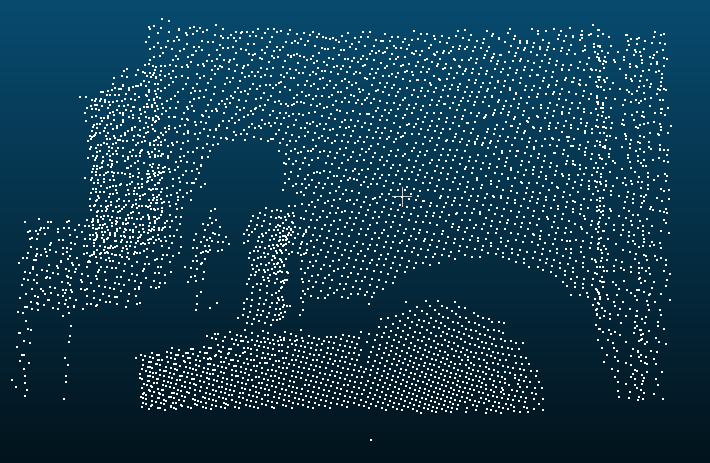
\includegraphics[width=.8\textwidth]{images/point-cloud-example.png}
		\caption{Point cloud generated from a test scene}
		\label{fig:point-cloud-input}
	\end{center}
\end{figure}

\begin{figure}[t]
	\begin{center}
		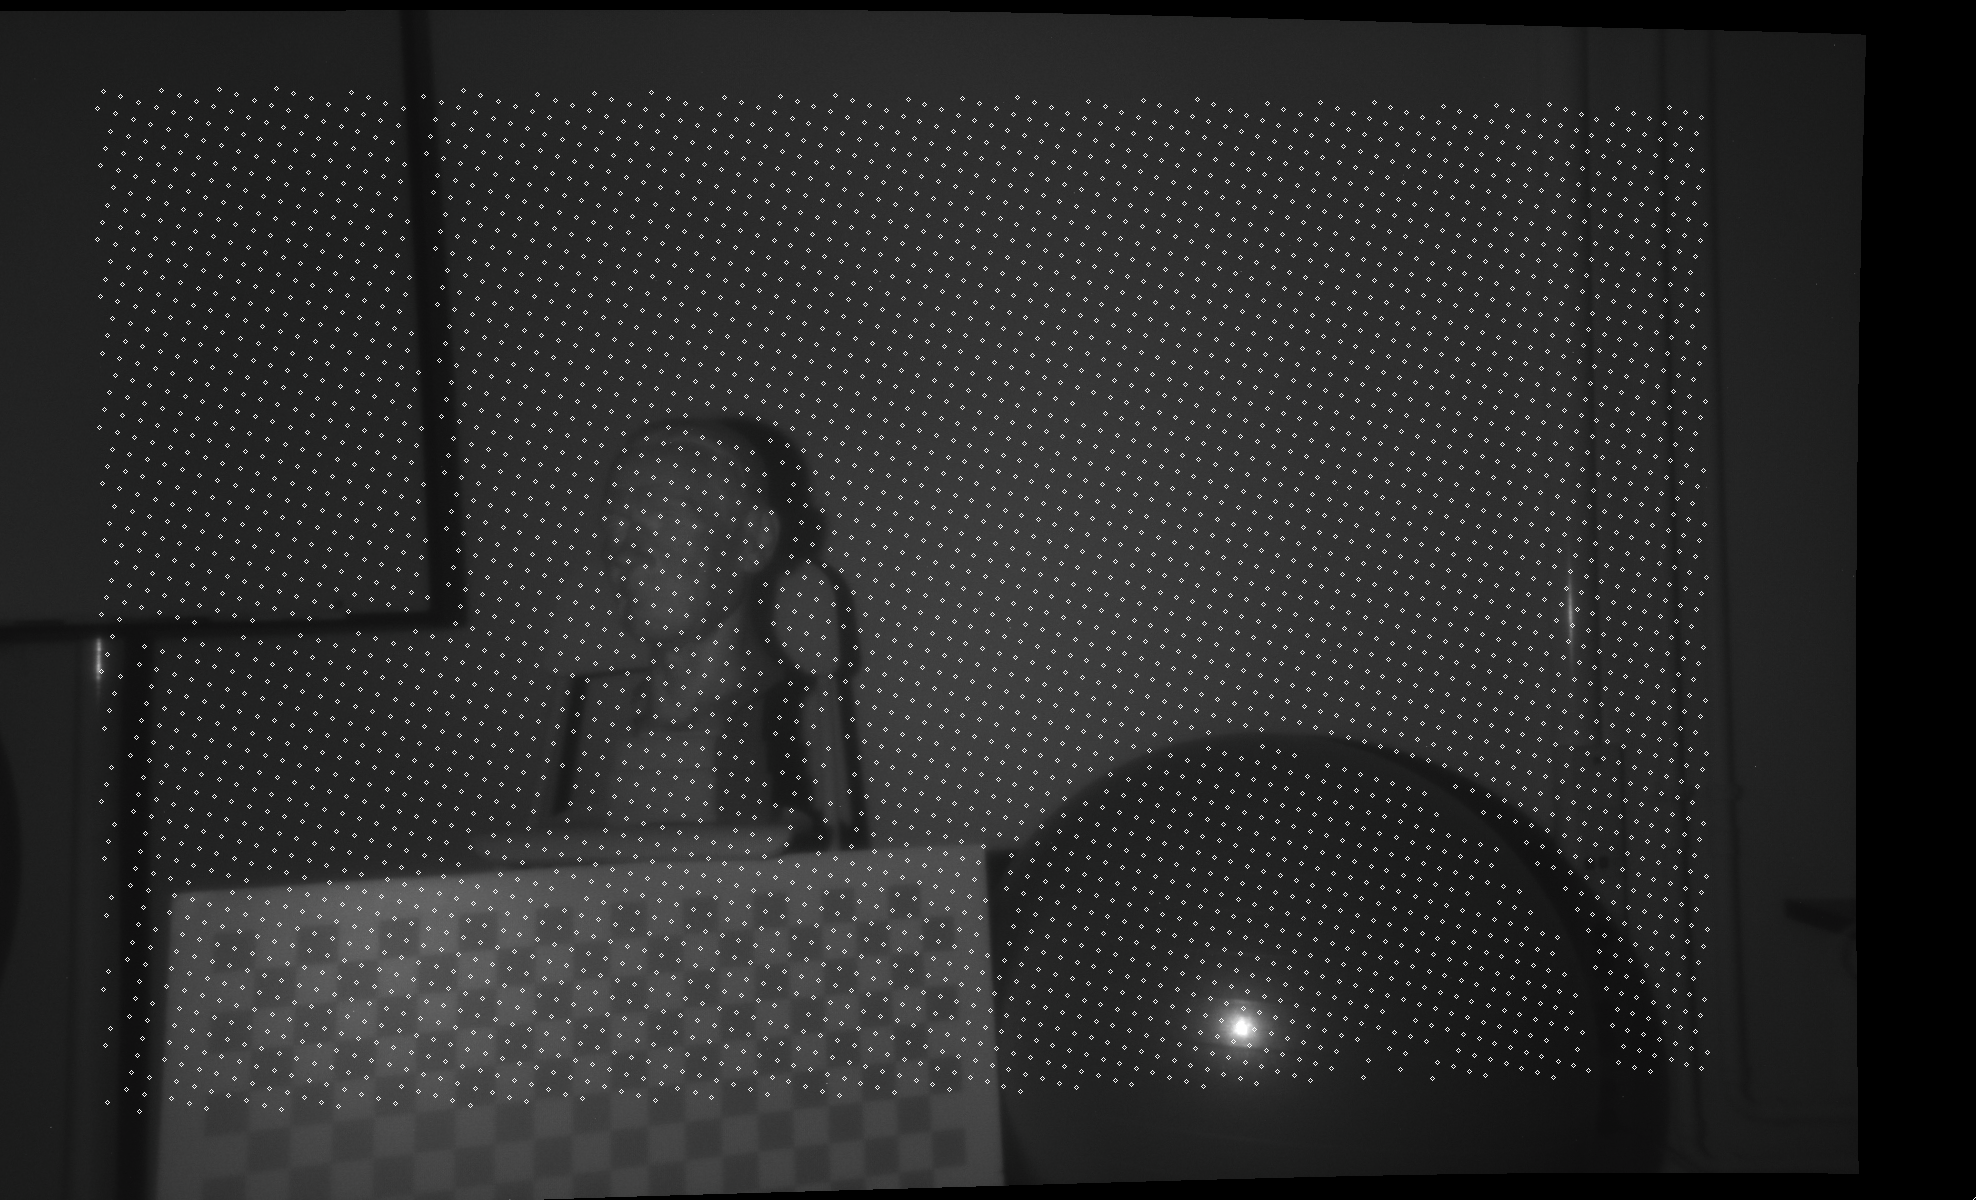
\includegraphics[width=.8\textwidth]{images/stereo-rectified-rgb.png}
		\caption{Primary stereo image with Ladimo grid point overlapped}
		\label{fig:primary-stereo-input}
	\end{center}
\end{figure}

One of the fundamental mainstay of this Master's Thesis project is the device developed by Ladimo, the company at which I am building up my project. 
Therefore, it is rather useful for a solid understanding of the work done for this thesis to describe, even briefly, the hardware designed by the company and its implementation in the developed work. \\
Ladimo device is structured light based 3D camera. 
Its core functionality is to output a 3D point cloud data of the analysed scene for the listening client. 
Technically speaking, the laser projector mounted on the device splits its beams into the affected area.
That set of laser points is then accurately measured by a camera \textbf{(or cameras)} sensitive to laser's wavelength.
Therefore, this system allows the user to generate a sparse grid of regularly separated points, which contain information on their 3D location, as visualized in Figure \ref{fig:point-cloud-input}. \\
So that, the described device can be exploited in order to improve in both accuracy and efficiency a stereo matching problem.
This is, indeed, the base of the study presented in this Master's thesis. 
In fact, as already deeply described in \ref{chapter:background}, one of the main drawbacks of creating a 3D dense point cloud using stereo matching techniques stands in the aggregation cost part. 
And that is closely related to the overall range of disparities associated to each stereo pair. 
Moreover, other key factors are the definition of the image, the amount of texture-less region contained in the analysed scene and the number of edges, which make the algorithms used in those processes even more complicated and computationally expensive. 
However, as visible in Figure \ref{fig:point-cloud-input} and \ref{fig:primary-stereo-input}, the laser grid generated with the Ladimo system cannot be considered enough dense to constitute an accurate 3D representation of the space. 
As a matter of fact, the points hit only some areas of the object and their sparsification does not allow to determine a continuous and smooth change between the surfaces of different objects, or even between different regions in the same object.
Furthermore, as extremely visible in the lower right-hand side of Figure \ref{fig:primary-stereo-input}, there are sections of the objects that almost completely lacks of points, usually in close proximity of occluded or shaded regions.\\
Therefore, an efficient strategy that can be applied to tackle the problem of creating a dense depth image from a pair of rectified stereo images is to exploit the initial piece of information contained in the grid points data. 
As a matter of fact, those data can be employed to make the overall pipeline of the algorithm more efficient. 
First of all, the error rate regarding wrong matches can be highly reduced, then, the disparity range over which the corresponding points are matched can be recursively selected basing on the disparity values of the neighbourhood of the analysed point. 
So that, these are only some of the improvement that can be applied to the process utilizing the information that comes from the Ladimo device.
Thus, as can be therefore understood, the Ladimo system was fundamental for the efficiency of the overall pipeline of the algorithm.
The different part of the algorithm and the achieved results will be deeply and precisely presented in the following chapters. 
As regards the current analysis of the work, it would be sufficient to introduce the general strategy applied and the reasons that lead to that decision.\\
Taking into account the output of the stereo device, it comprises the two stereo images of the scene, which have to be rectified in order to have the corresponding point along the same epipolar line, and the grid of points generated from the laser projector. 
Regarding the laser grid, as can be understood from the brief system description, it can be correctly recovered for one of the images only. 
As a matter of fact, the grid points are thus overlapped with the primary image, usually the left one. 
This configuration is, thus, exploited to run the entire pipeline. 
Moreover, it would be also possible to define the corresponding grid for the right image, employing the camera matrix parameters. 
So that, a second reciprocal pipeline could be carried out in parallel. 
In this manner, two different dense depth map are obtained and then handled to apply specific post-processing procedures such as left-right consistency check, which allow to determine possible wrong matches and especially occluded pixel depth values. 
As aforementioned, the corresponding coordinates of the points can be recovered exploiting the camera matrix parameters, which allow to build up a second grid over the support image. 
However, this phase is not completely necessary for the main purpose of the designed stereo matching algorithm.
It will allow to perform specific and accurate post-processing procedures. 
Nevertheless, this has to be evaluated in terms of desired accuracy and computational time, considering that, even simpler post-processing techniques, such as morphological or median filters has shown to give an accurate enough 3D dense point cloud.\\


\section{Software Environment}
\label{section:software-env}

Considering the programming related part of the built environment, it comprises multiple software and platforms. 
Although, some computing environments and frameworks were not entirely employed during the overall designing of the project, this was due to the decisions correlated to the way in which the work was conceived and the choices regarding the applicable strategy. \\
As a matter of fact, in the initial phase different methods and approaches have been tested using MATLAB\footnote{The software was used for academic purposes being available through the personal university account}. 
Despite the known fact that further working implementation of the algorithm would not be run using an academic version of the aforementioned software, a first researching phase was initially planned.
Multiple reasons support that decision, such as a personal considerable knowledge of the software and of its built-in libraries and functions, the possibility to check the results of the performed tests in an user-friendly manner and the side own need to get confidence with the company's hardware and software environment.\\
Taking those choices into account, the initial part of the work was dedicated to research and tests necessary to evaluate the proper strategy for the algorithm development and to conduct comparisons between some initial ideas and a bunch of available methods.\\


\subsection{MATLAB computing environment}
\label{subsection:matlab-env}
As introduced above, primary tests have been handles using MATLAB\textsuperscript{\textregistered} and especially some built-in functions correlated to stereo matching and image manipulation.\\
MATLAB can be defined as a platform composed of a multi-paradigm\footnote{functional, imperative, procedural, object-oriented, array} numerical computing environment and a proprietary programming language created by MathWorks.
It is significantly used for matrix manipulation, algorithm implementation and plotting of data and functions.
Moreover, one of its most utilized packages is Simulink, which allows the user to develop even extremely complex algorithms, especially for dynamic and embedded systems, with a block-based interface. \\
Although its high versatility and possibility to design programs that can be run of different systems, it was decided not to make it the main environment of the project, in order to not be limited from both a software and patent perspectives.\\
Consequently, after the initial preparatory phase of the project, the primary development of the algorithm has been realized through a C++ code, which has been built up using Microsoft Visual Studio and the OpenCV library. 

\subsection{Microsoft Visual Studio integrated development environment}
\label{subsection:visual-studio-env}

Microsoft Visual Studio is an integrated development environment (IDE) crated by Microsoft. 
It is used for several purposes, such as software development, websites, web services, mobile as well as web applications. 
Obviously, it is based on Microsoft software development platforms, e.g. Windows API, Windows Form and Windows Presentation Foundation. 
It is also advisable to mention some of its assets, which make it the most preferred IDE, in terms of popularity\footnote{According to data from Google Trends and available at \url{https://pypl.github.io/IDE.html}}. \\
First of all, it allows to create both native, or machine language, code and managed code.
Moreover, among its most powerful features there are IntelliSense, the intelligent code completion included in the editor, and the integrated debugger, which operates both as source-level debugger and a machine-level debugger. 
Furthermore, it contains lot of other built-in tools, designed for multiple applications and objectives, plug-ins that enhance coding capabilities and it supports almost any programming language.\\
Considering specifically its architecture, it actually does not support inherently any programming language, solution or tool.
Rather, it permits the integration of functionalities coded as VSPackage, i.e. Visual Studio Package, which are software modules that broaden the Visual Studio IDE by supplying UI elements, services, projects, editors and designers. 
Therefore, at its native behaviour, it works as a \textit{Service} solution. 
As an example, the support for programming language is added by using a specific VSPackage knows as \textit{Language Service}.
Exploiting that service various functionalities can be included in the IDE. 

\subsection{C++ programming language}
\label{subsection:c++-env}

Subsequently to the initial preparatory phase, in which the main employed environment was MATLAB, the actual design of the final algorithm has been developed basing on the C++ syntax.\\
The decision of exploiting MATLAB only for the initial planning of the work and for the first tests correlated to the feasibility of the various ideas was mainly due to multiple reasons, which cover different aspects of the entire design of the project.
First of all, since the beginning there was the intention of designing an algorithm that would be adaptable to different types of hardware and which would be further adjusted to other programming languages, e.g. CUDA, in order to obtain better final performances.
Moreover, considering plausible forthcoming commercial issues, there was the need to ensure a developing as free from copyright as possible. 
Flexibility and efficiency were other fundamental drivers of that choice. 
As widely know in the technological field, C++ programming language can ensure velocity and efficiency of the designed software as well as flexibility with different types of hardware.
In fact, it can be optimal for coding both at high levels of abstraction, and at low levels, e.g. at machine language level.
Then, in relation with this very project implementation, using C++ was possible to widely exploit the functions of the OpenCV library. \\
Therefore, adopting C++ as the fundamental programming language of this Master's Thesis project, it was possible to reach a sufficient level of computational speed, trying to minimize the memory requirements and simultaneously keep a high amount of abstraction, necessary for working effectively in the computer vision field. 


\subsection{OpenCV cross-platform library}
\label{subsection:opencv-env}

OpenCV, Open Source Computer Vision Library, is a library of programming algorithms primarily intended at real-time computer vision.\\
It was employed as a fundamental support structure of this project mainly because of the functions accessible in that library, the fact that is open source and the remarkable documentation available. 
Moreover, thanks to those algorithms, the implementation of methods and functions inside the project pipeline became faster, more reliable and multiple pre-processing and post-processing techniques has been tested, following structural changing in the main algorithm.\\
Therefore, OpenCV library can be considered as an important resource of this work.
For that, and for more theoretical purposes, it appropriate to introduce the main feature of that computer vision based library.\\
First of all, OpenCV was initially developed by Intel, then later maintained by Willow Garage, a robotic research lab and technology incubator and subsequently by Itseez, currently acquired by Intel.
Precisely, the library is cross-platform and open-source, under BSD, Berkeley Software Distribution, license. 
The library was initially created to advance CPU-intensive applications, related to real-time tracing and 3D display walls project.
Considering that, it is therefore clear why it is widely exploited when dealing with computer vision correlated works.\\
As defined in \cite{bradski2008learning}, the main targets of the initial project were:
\begin{itemize}
	\item Accelerate vision research providing open and optimized code for essential vision framework.
	\item Aim for a more readable and interchangeable code by providing a universal infrastructure to use.
	\item Enhance vision-based commercial projects by producing a portable and optimized code available with a free license.
\end{itemize}
Currently, OpenCV library is one of the most used platform by mainly computer software companies.
As a matter of fact, it has been calculated that it counts more than 47 thousand people of user community and an evaluated number of downloads surpassing 18 million \footnote{Data from \url{https://opencv.org/about/}}.\\
Thus, it has been chosen as one of the main assets of the developed work, because of the aforementioned reasons, and in relation to the available applications, which can be used in multiple computer vision related areas, such as, 2D and 3D feature toolkits, facial recognition systems, mobile robotics, object detection, segmentation and recognition and diverse machine learning fields.


\subsection{CloudCompare 3D editing and processing software}
\label{subsection:cloud-compare-env}

CloudCompare is a software that was exploited during this project almost exclusively for the accurate 3D point cloud visualization, which it can easily provide.
Therefore, it can be considered as a side software used in this work, which help to get coherent visualizations of the result, things that results difficult or overcomplicated employing OpenCV functions and C++. 
On the contrary, with this software was easy to visualize the computed results, and deeply understand if the modifications made in the code works correctly, improving the final results.\\
Therefore, to provide a brief presentation of this software, it is basically a 3D point cloud processing software.
Originally, it was developed to operate comparison between two dense 3D points clouds, such as the ones collected with laser scanner, or between a point cloud and a triangular mesh.
On top of that, it has been further expand to a more multi-purposes point cloud processing software, providing multiple advanced algorithms for data handling and processing. 



 
